% !Mode:: "TeX:UTF-8"
\chapter{开发环境}

\begin{introduction}
	\item 开发环境
	\item 安装JDK
	\item 安装IDE
\end{introduction}

本书使用Java语言介绍机器学算法,所有的演示代码可在JDK8以上正常运行。
在开始学习之前,请先安装JDK(Java Development Kit)和IDE(Integrated Development Environment)。

\begin{table}[!htbp]\centering
	\caption{开发环境}
	\begin{tabular}{|p{1cm}|p{3cm}|p{8cm}|}
	\toprule
	序号 & \multicolumn{2}{|c|}{开发环境}\\
	\midrule
	1. & JDK8+&建议Oracle JDK\\
	\hline
	2. & IntelliJ IDEA&界面友好,操作简单\\
	\hline
	3. & VSCode&强大开源,插件众多\\
	\hline
	4. & ND4J&Java实现的矩阵/向量支持库\\
	\hline
	5. & DL4J&开源机器学习Java实现\\
	\bottomrule
	\end{tabular}
\end{table}

\section{安装JDK}
你有2个选择:Oracle JDK和Open JDK,实际上你可以无视它们之间的差异。
使用Linux系统的同学,安装Open JDK即可。
值得注意的是,近年来关于Oracle JDK的纠纷越来越多,
实际上,在Sun被Oracle收购之前,JDK也是要授权费的,但很少有公司愿意支付这笔费用。
\bigskip
\begin{table}[!htbp]\centering \small
	\begin{tabular}{cc|c|ccc|c|cc}
		\toprule
		输入&&编译&&输出&&执行&&输出 \\
		\midrule
		Hello.java&=>&javac&=>&Hello.class&=>&java&=>&输出 \\
		&&JDK&&&&JRE&& \\
		\bottomrule
	\end{tabular}
\end{table}

开发需要安装Java Development Kit,而JRE(Java Runtime Environment)是Java程序的运行环境,不要下载错了。
JDK的安装包有两种方式:压缩包、安装文件,优先下载安装包,全部默认“下一步”即可。
如果是压缩包,理论上解压到任何位置都可以,不过建议常用位置。
\footnote{官网在/usr/java/目录下解压jdk压缩包,或者/usr/lib/jvm/也很常见。}
结束后,需要手动配置以下2个环境变量:JAVA\_HOME、CLASSPATH。
配置环境变量的主要目的是告诉IDE或系统,在哪里能找到某个程序或文件。
把JAVA\_HOME
设定为JDK的安装目录,进一步在此基础上添加bin目录到环境变量。
如果没有配置,或者设置不正确,在控制台(cmd、bash)就会提示错误。
\begin{lstlisting}[language=bash]
	# Ubuntu
	parallels@ubuntu-vm:~$ java
	Command 'java' not found, but can be installed with:

	# Windows
	C:\Users\simbaba>java
	'java' 不是内部或外部命令,也不是可运行的程序
	或批处理文件。
\end{lstlisting}

Windows上的配置相对比较简单,参考下图打开环境变量配置窗口。
选择系统环境变量或者帐号环境变量里面都可以,区别是系统环境变量会影响所有用户。
通常建议修改帐号环境变量,有些帐号可能也没权限修改系统环境变量。

\begin{figure}[!htb]
	\centerline{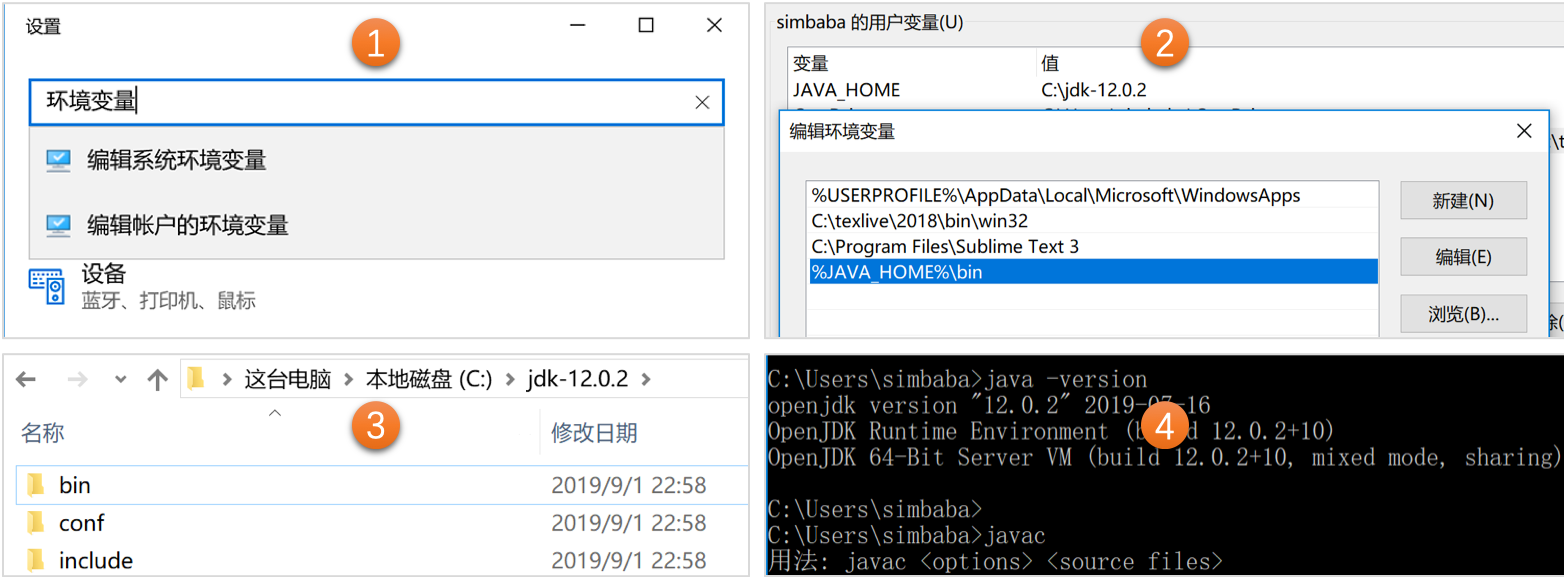
\includegraphics[scale=.7]{images/windows_java_set.png}}
\end{figure}

\remark{Linux和Mac的配资方法大致相同,需要修改配置文件。}
\footnote{.bash\_profile、.bashrc或.profile等。}
\begin{lstlisting}[language=bash]
	# Mac、Linux
	export JAVA_HOME= JAVA安装目录
	export path=$PATH:$JAVA_HOME/bin
\end{lstlisting}

配置CLASS\_PATH的操作与上述步骤相同,但目前不需要配置,我们会在后面对此进行介绍。
使用IDE的同学,完全可以忽略这个配置。

\section{安装IDE}
当前主流的IDE有:Eclipse、IDEA、VSCode。
好用的IDE不仅有助于提高编码效率,还可以辅助检查学习过程中的错误。
根据个人喜好选择一个即可,本书例子全部在VSCode上验证通过。

\begin{figure}[!htb]
	\centering
	\begin{minipage}{0.2\textwidth}
		
\includegraphics[width=2cm]{images/logo_eclipse.png} \\
		\centering Eclipse
	\end{minipage}
	\begin{minipage}{0.2\textwidth}
		
\includegraphics[width=2cm]{images/logo_vscode.png} \\
		\centering VS Code
	\end{minipage}
	\begin{minipage}{0.2\textwidth}
		
\includegraphics[width=2cm]{images/logo_idea.png} \\
		\centering IDEA
	\end{minipage}
\end{figure}

实际上,对于初学者不使用IDE才能了解更多细节,限于本书篇幅在此不做过多论述。
IDEA安装社区版本即可,专业版需要付费,但也不建议使用破解版。
如果动手能力强的同学,建议使用VSCode。

\section{安装git}
使用版本控制工具,可以帮助你管理代码。
你的每一次提交都将生成一个记录,方便回退和合并代码。
你发布的每一个软件版本,也都会记录在代码仓库的标签上。

\begin{figure}[!htb]
	\centerline{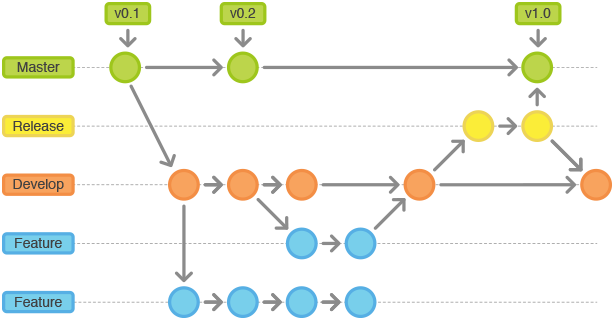
\includegraphics[scale=.8]{images/git-workflow.png}}
\end{figure}

在软件开发中,分解出许多小的Feature需要实现。
首先,我们创建一个Master分支,然后基于此拉一个Develop分支。
以后,发布正式版本的时候,就基于Develop拉出一个Release分支做验证。
验证不通过,还会做一些修改,最终合并到Master分支和Develop分支。
所有的Feature开发都在Develop分支基础上拉出一个基线,
待开发完成之后,把该Feature代码合入Develop分支。
等到Develop分支合入足够多Feature之后,就可以发布版本。

git的安装比较简单,使用Windows的同学可在\url{https://git-scm.com/}下载安装。
其它操作系统,可使用apt-get(Ubuntu)、brew(Mac)安装git。
如果不能在cmd、bash上使用git,请参照之前内容配置环境变量。
git的使用方法不在此赘述,请参照其它书籍学习。
掌握git init, git add, git commit, git push基本就可以了。
对于git branch之类更高级的使用方法,可以暂时不掌握。